
\documentclass{beamer}

\usepackage{framed}
\usepackage{graphicx}

\begin{document}
\section{Visualizing linear relationships}
%=========================================%
\begin{frame}
	\begin{itemize}
		\item
		Many datasets contain multiple quantitative variables, and the goal of an analysis is often to relate those variables to each other. \item We previously discussed functions that can accomplish this by showing the joint distribution of two variables. It can be very helpful, though, to use statistical models to estimate a simple relationship between two noisy sets of observations. \item The functions discussed in this chapter will do so through the common framework of linear regression.
		\end{itemize}
\end{frame}
%=========================================%
\begin{frame}
	\begin{itemize}
\item In the spirit of Tukey, the regression plots in seaborn are primarily intended to add a visual guide that helps to emphasize patterns in a dataset during exploratory data analyses. 
\item That is to say that seaborn is not itself a package for statistical analysis. To obtain quantitative measures related to the fit of regression models, you should use statsmodels. 
\item The goal of seaborn, however, is to make exploring a dataset through visualization quick and easy, as doing so is just as (if not more) important than exploring a dataset through tables of statistics.
	\end{itemize}

\end{frame}
%=========================================%
\begin{frame}[fragile]
	\begin{verbatim}
%matplotlib inline
import numpy as np
import pandas as pd
import matplotlib as mpl
import matplotlib.pyplot as plt
import seaborn as sns
sns.set(color_codes=True)
np.random.seed(sum(map(ord, "regression")))
tips = sns.load_dataset("tips")
	\end{verbatim}

\end{frame}
%========================================================%
\subsection{Functions to draw linear regression models}
\begin{frame}
Two main functions in seaborn are used to visualize a linear relationship as determined through regression. These functions, regplot() and lmplot() are closely related, and share much of their core functionality. It is important to understand the ways they differ, however, so that you can quickly choose the correct tool for particular job.
\end{frame}
%===================================================================== %
\begin{frame}[fragile]
	\frametitle{Seaborn Workshop}
	\large
In the simplest invocation, both functions draw a scatterplot of two variables, x and y, and then fit the regression model y ~ x and plot the resulting regression line and a 95\% confidence interval for that regression:
\end{frame}
%===================================================================== %
\begin{frame}[fragile]
	\frametitle{Seaborn Workshop}
	\large
\begin{verbatim}
sns.regplot(x="total_bill", y="tip", data=tips);
\end{verbatim}

\begin{figure}
	\centering
	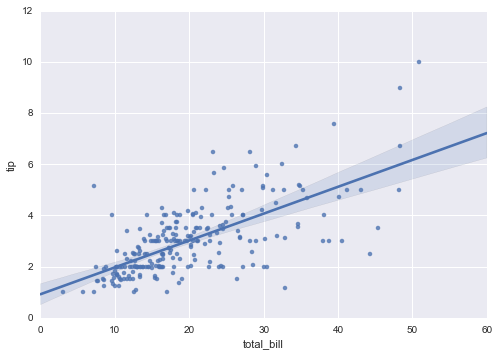
\includegraphics[width=0.7\linewidth]{images/regression_9_0}
\end{figure}
\end{frame}
%===================================================================== %
\begin{frame}[fragile]
	\frametitle{Seaborn Workshop}
	\large
\begin{verbatim}
sns.lmplot(x="total_bill", y="tip", data=tips);
\end{verbatim}
\begin{figure}
	\centering
	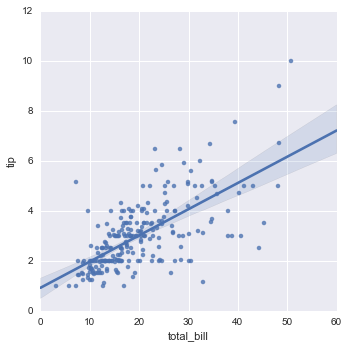
\includegraphics[width=0.7\linewidth]{images/regression_10_0}
\end{figure}
\end{frame}
%===================================================================== %
\begin{frame}[fragile]
	\frametitle{Seaborn Workshop}
	\large
You should note that the resulting plots are identical, except that the figure shapes are different. We will explain why this is shortly. For now, the other main difference to know about is that regplot() accepts the x and y variables in a variety of formats including simple numpy arrays, pandas Series objects, or as references to variables in a pandas DataFrame object passed to data. In contrast, \texttt{lmplot()} has data as a required parameter and the x and y variables must be specified as strings. 

\end{frame}
%===================================================================== %
\begin{frame}[fragile]
	\large
	
\begin{itemize}
\item This data format is called “long-form” or “tidy” data. Other than this input flexibility, \texttt{regplot()} possesses a subset of \texttt{lmplot()}‘s features, so we will demonstrate them using the latter.

\item It’s possible to fit a linear regression when one of the variables takes discrete values, however, the simple scatterplot produced by this kind of dataset is often not optimal:
\end{itemize}
\end{frame}
%===================================================================== %
\begin{frame}[fragile]
	\large
	
sns.lmplot(x="size", y="tip", data=tips);
\begin{figure}
	\centering
	\includegraphics[width=0.7\linewidth]{images/regression_12_0}
\end{figure}
\end{frame}
%===================================================================== %
\begin{frame}[fragile]
	\large
One option is to add some random noise (“jitter”) to the discrete values to make the distribution of those values more clear. Note that jitter is applied only to the scatterplot data and does not influence the regression line fit itself:
\begin{framed}
\begin{verbatim}
sns.lmplot(x="size", y="tip", data=tips, x_jitter=.05);
\end{verbatim}
\end{framed}/
\begin{figure}
\centering
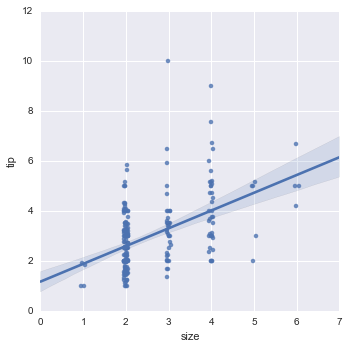
\includegraphics[width=0.7\linewidth]{images/regression_14_0}
\end{figure}


\end{frame}
%===================================================================== %
\begin{frame}[fragile]
	\large
A second option is to collapse over the observations in each discrete bin to plot an estimate of central tendency along with a confidence interval:
\begin{verbatim}
sns.lmplot(x="size", y="tip", data=tips, x_estimator=np.mean);
\end{verbatim}

\begin{figure}
\centering
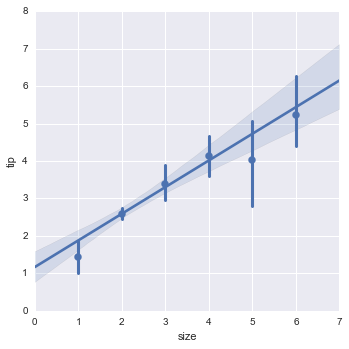
\includegraphics[width=0.7\linewidth]{images/regression_16_0}
\caption{}
\label{fig:regression_16_0}
\end{figure}


\end{frame}
\section{Visualizing Linear Relationships}
\begin{frame}
	\frametitle{Seaborn : Visualizing Linear Relationships}
	\large
	\begin{itemize}
		\item The simple linear regression model used above is very simple to fit, however, it is not appropriate for some kinds of datasets. 
		\item The Anscombe’s quartet dataset shows a few examples where simple linear regression provides an identical estimate of a relationship where simple visual inspection clearly shows differences. 
		\item For example, in the first case, the linear regression is a good model:
	\end{itemize}
\end{frame}
%======================================================= %
\begin{frame}[fragile]
	\frametitle{Seaborn : Visualizing Linear Relationships}
	\large
	\begin{framed}
		\begin{verbatim}
		anscombe = sns.load_dataset("anscombe")
		sns.lmplot(x="x", y="y", data=anscombe.query("dataset == 'I'"),
		ci=None, scatter_kws={"s": 80});
		\end{verbatim}
	\end{framed}
\end{frame}

%=========================================%
\begin{frame}[fragile]
	\frametitle{Seaborn : Visualizing Linear Relationships}
	\large	
	\begin{figure}
		\centering
		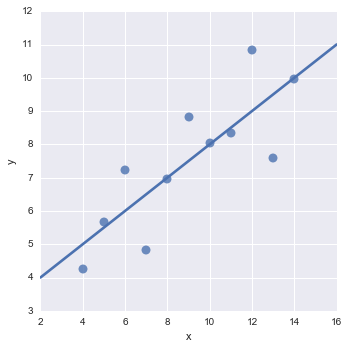
\includegraphics[width=0.7\linewidth]{images/regression_19_0}
	\end{figure}
	
\end{frame}

%=========================================%
\begin{frame}[fragile]
	\frametitle{Seaborn : Visualizing Linear Relationships}
	\large	
	The linear relationship in the second dataset is the same, but the plot clearly shows that this is not a good model:
	\begin{framed}
		\begin{verbatim}
		sns.lmplot(x="x", y="y", 
		data=anscombe.query("dataset == 'II'"),
		ci=None, scatter_kws={"s": 80});
		\end{verbatim}
	\end{framed}
	\begin{figure}
		\centering
		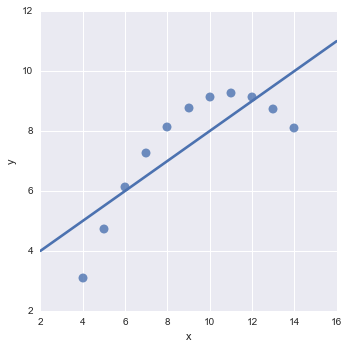
\includegraphics[width=0.7\linewidth]{images/regression_21_0}
	\end{figure}
	
	
\end{frame}


%=========================================%
\begin{frame}[fragile]
	\frametitle{Seaborn : Visualizing Linear Relationships}
	\large	
	In the presence of these kind of higher-order relationships, \texttt{lmplot()} and \texttt{regplot()} can fit a polynomial regression model to explore simple kinds of nonlinear trends in the dataset:
	
\end{frame}
%=========================================%
\begin{frame}[fragile]
	\frametitle{Seaborn : Visualizing Linear Relationships}
	\large
	\begin{framed}
		\begin{verbatim}
		sns.lmplot(x="x", y="y", 
		data=anscombe.query("dataset == 'II'"),
		order=2, ci=None, scatter_kws={"s": 80});
		\end{verbatim}
	\end{framed}
	\begin{figure}
		\centering
		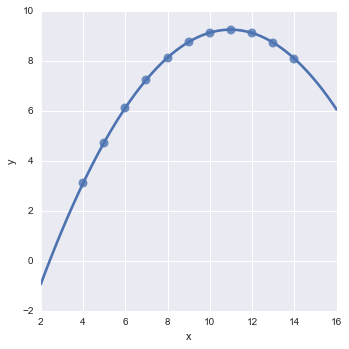
\includegraphics[width=0.55\linewidth]{images/regression_23_0}
		
	\end{figure}
	
\end{frame}
%=========================================%
\begin{frame}[fragile]
	\frametitle{Seaborn : Visualizing Linear Relationships}
	\large
	A different problem is posed by “outlier” observations that deviate for some reason other than the main relationship under study:
	\begin{framed}
		\begin{verbatim}
		sns.lmplot(x="x", y="y", data=anscombe.query("dataset == 'III'"),
		ci=None, scatter_kws={"s": 80});
		\end{verbatim}
	\end{framed}
	\begin{figure}
		\centering
		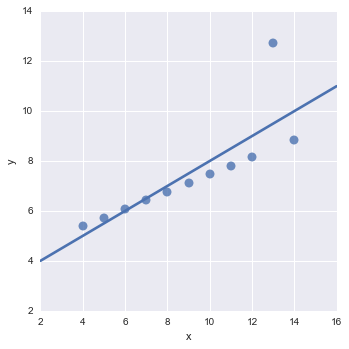
\includegraphics[width=0.55\linewidth]{images/regression_25_0}
	\end{figure}
	
	
\end{frame}
%=========================================%
\begin{frame}[fragile]
	\frametitle{Seaborn : Visualizing Linear Relationships}
	\large
	In the presence of outliers, it can be useful to fit a robust regression, which uses a different loss function to downweight relatively large residuals:
	\begin{framed}
		\begin{verbatim}
		sns.lmplot(x="x", y="y", data=anscombe.query("dataset == 'III'"),
		robust=True, ci=None, scatter_kws={"s": 80});
		\end{verbatim}
	\end{framed}
	\begin{figure}
		\centering
		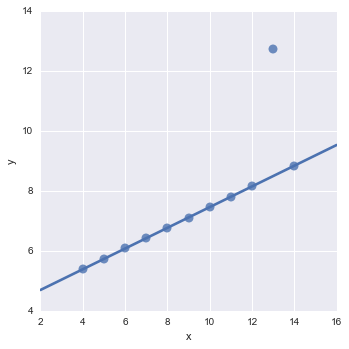
\includegraphics[width=0.55\linewidth]{images/regression_27_0}
		
	\end{figure}
\end{frame}
%=========================================%
\begin{frame}[fragile]
	\frametitle{Seaborn : Visualizing Linear Relationships}
	When the y variable is binary, simple linear regression also “works” but provides implausible predictions:
	\begin{verbatim}
	tips["big_tip"] = (tips.tip / tips.total_bill) > .15
	sns.lmplot(x="total_bill", y="big_tip", data=tips,
	y_jitter=.03);
	\end{verbatim}
	\begin{figure}
		\centering
		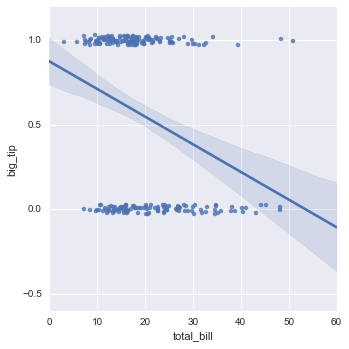
\includegraphics[width=0.55\linewidth]{images/regression_29_0}
	\end{figure}
	
\end{frame}
%=========================================%
\begin{frame}[fragile]
	\frametitle{Seaborn : Visualizing Linear Relationships}
	The solution in this case is to fit a logistic regression, such that the regression line shows the estimated probability of y = 1 for a given value of x:
	\begin{verbatim}
	sns.lmplot(x="total_bill", y="big_tip", data=tips,
	logistic=True, y_jitter=.03);
	\end{verbatim}
	\begin{figure}
		\centering
		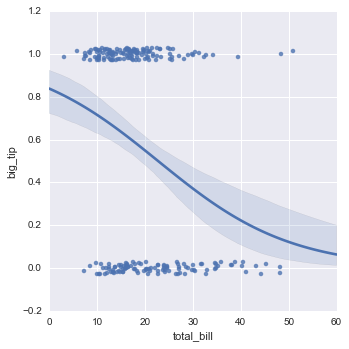
\includegraphics[width=0.55\linewidth]{images/regression_31_0}
	\end{figure}
\end{frame}
%===========================================================%
\begin{frame}
	\frametitle{Seaborn : Visualizing Linear Relationships}
	\large
	\begin{itemize}
		\item Note that the logistic regression estimate is considerably more computationally intensive (this is true of robust regression as well) than simple regression, and as the confidence interval around the regression line is computed using a bootstrap procedure, you may wish to turn this off for faster iteration (using \texttt{ci=False}).
		\item An altogether different approach is to fit a nonparametric regression using a lowess smoother. This approach has the fewest assumptions, although it is computationally intensive and so currently confidence intervals are not computed at all:
	\end{itemize}
	
	
\end{frame}
%==============================================%
\begin{frame}[fragile]
	\frametitle{Seaborn : Visualizing Linear Relationships}
	\large
	
	\begin{verbatim}
	sns.lmplot(x="total_bill", y="tip", data=tips,
	lowess=True);
	\end{verbatim}
	\begin{figure}
		\centering
		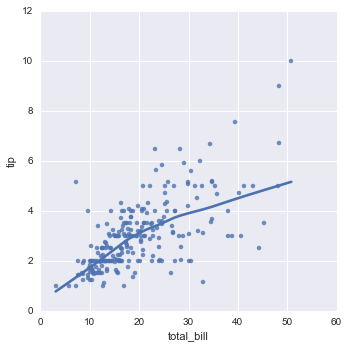
\includegraphics[width=0.55\linewidth]{images/regression_33_0}
	\end{figure}
	
\end{frame}
%==============================================%
\begin{frame}[fragile]
	\frametitle{Seaborn : Visualizing Linear Relationships}
	\large
	\begin{itemize}
		\item The \texttt{residplot()} function can be a useful tool for checking whether the simple regression model is appropriate for a dataset. 
		\item It fits and removes a simple linear regression and then plots the residual values for each observation. 
		\item Ideally, these values should be randomly scattered around \texttt{y = 0}:
	\end{itemize}	
	
	
\end{frame}
%==============================================%
\begin{frame}[fragile]
	\frametitle{Seaborn : Visualizing Linear Relationships}
	\large
	\begin{verbatim}
	sns.residplot(x="x", y="y", data=anscombe.query("dataset == 'I'"),
	scatter_kws={"s": 80});
	\end{verbatim}
	
	\begin{figure}
		\centering
		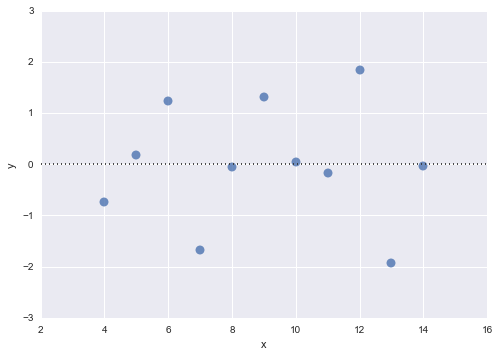
\includegraphics[width=0.7\linewidth]{images/regression_35_0}
	\end{figure}
\end{frame}
%==============================================%
\begin{frame}[fragile]
	\frametitle{Seaborn : Visualizing Linear Relationships}
	\large
	If there is structure in the residuals, it suggests that simple linear regression is not appropriate:
	\begin{verbatim}
	sns.residplot(x="x", y="y", data=anscombe.query("dataset == 'II'"),
	scatter_kws={"s": 80});
	\end{verbatim}
	\begin{figure}
		\centering
		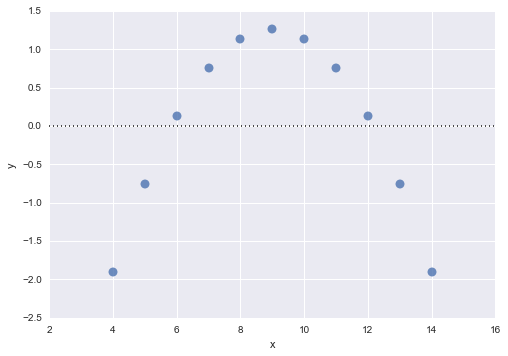
\includegraphics[width=0.7\linewidth]{images/regression_37_0}
	\end{figure}
	
\end{frame}
%============================================================%
\section{Conditioning on other variables}
\begin{frame}
	\frametitle{Seaborn Workshop}
	\large
	\textbf{Conditioning on other variables}
	\begin{itemize}
		\item The plots above show many ways to explore the relationship between a pair of variables.
		\item Often, however, a more interesting question is “how does the relationship between these two variables change as a function of a third variable?” 
		\item This is where the difference between \texttt{regplot()} and \texttt{lmplot()} appears. 
		\item While \texttt{regplot()} always shows a single relationsihp, \texttt{lmplot()} combines \texttt{regplot()} with FacetGrid to provide an easy interface to show a linear regression on “faceted” plots that allow you to explore interactions with up to three additional categorical variables.
	\end{itemize}
	
\end{frame}
%===========================================================%
\begin{frame}[fragile]
	\frametitle{Seaborn Workshop}
	\large
	
	The best way to separate out a relationship is to plot both levels on the same axes and to use color to distinguish them:
	\begin{verbatim}
	sns.lmplot(x="total_bill", y="tip", 
	hue="smoker", data=tips);
	\end{verbatim}
	
	\begin{figure}
		\centering
		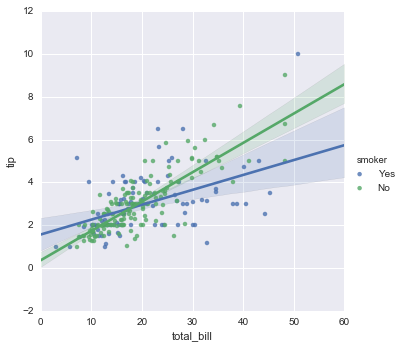
\includegraphics[width=0.55\linewidth]{images/regression_39_0}
	\end{figure}
\end{frame}
%===========================================================%
\begin{frame}[fragile]
	\frametitle{Seaborn Workshop}
	\large
	
	In addition to color, it’s possible to use different scatterplot markers to make plots the reproduce to black and white better. You also have full control over the colors used:
	\begin{verbatim}
	sns.lmplot(x="total_bill", y="tip", hue="smoker", data=tips,
	markers=["o", "x"], palette="Set1");
	\end{verbatim}
	\begin{figure}
		\centering
		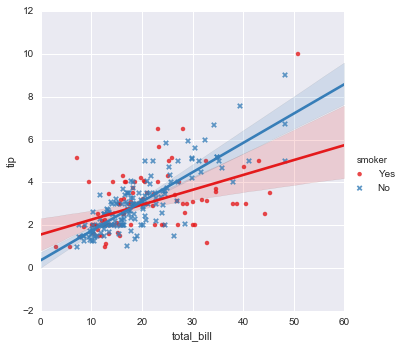
\includegraphics[width=0.7\linewidth]{images/regression_41_0}
	\end{figure}
\end{frame}
%==============================================%
\begin{frame}[fragile]
	\large
	To add another variable, you can draw multiple “facets” which each level of the variable appearing in the rows or columns of the grid:
	\begin{verbatim}
	sns.lmplot(x="total_bill", y="tip", 
	hue="smoker", col="time", 
	data=tips);
	\end{verbatim}
	
	\begin{figure}
		\centering
		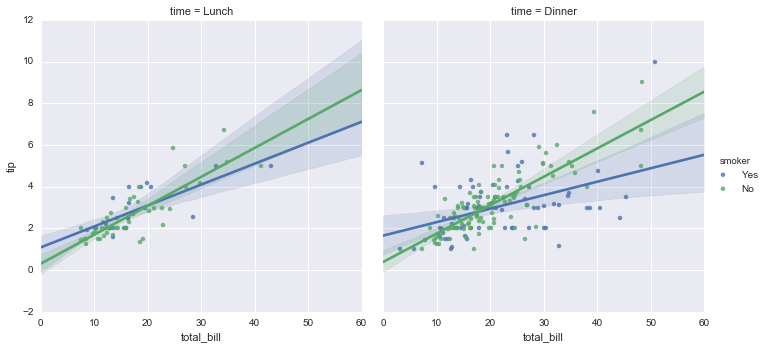
\includegraphics[width=0.55\linewidth]{images/regression_43_0}
	\end{figure}
	
\end{frame}
%===========================================================%
\begin{frame}[fragile]
	\frametitle{Seaborn Workshop}
	\large
	\begin{verbatim}
	sns.lmplot(x="total_bill", y="tip", hue="smoker",
	col="time", row="sex", data=tips);
	\end{verbatim}
	
	\begin{figure}
		\centering
		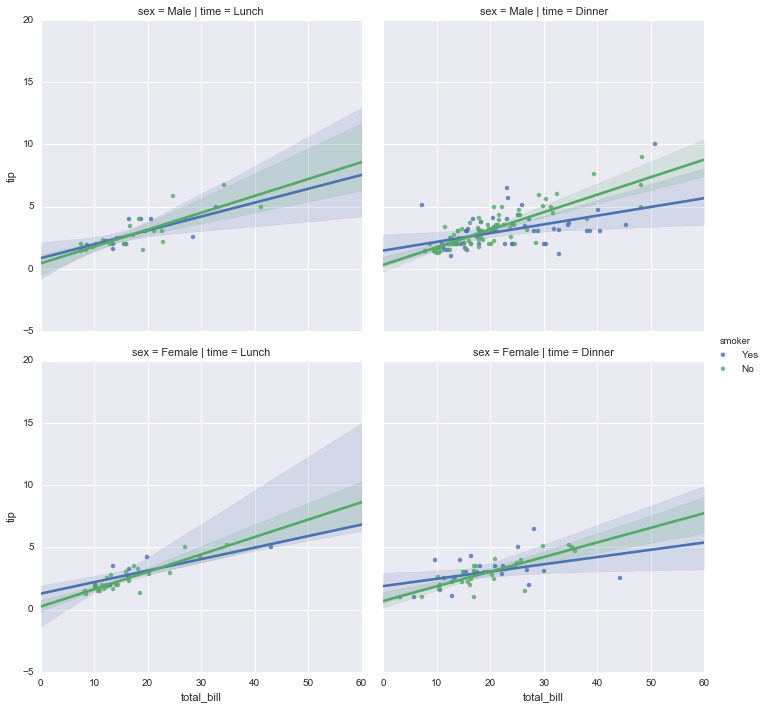
\includegraphics[width=0.7\linewidth]{images/regression_44_0}
	\end{figure}
\end{frame}
%=============================================================%
\section{Controlling the size and shape of the plot}
\begin{frame}[fragile]
	\frametitle{Seaborn Workshop}
	\large
	\begin{itemize}
		\item Before we noted that the default plots made by \texttt{regplot()} and \texttt{lmplot()} look the same but on axes that have a different size and shape. This is because func:regplot is an “axes-level” function draws onto a specific axes.
		\item  This means that you can make mutli-panel figures yourself and control exactly where the the regression plot goes. 
		\item If no axes is provided, it simply uses the “\textit{currently active}” axes, which is why the default plot has the same size and shape as most other matplotlib functions. To control the size, you need to create a figure object yourself.
	\end{itemize}
	
\end{frame}
%=========================================%
\begin{frame}[fragile]
	\frametitle{Seaborn Workshop}
	\large
	\begin{framed}
		\begin{verbatim}
		f, ax = plt.subplots(figsize=(5, 6))
		sns.regplot(x="total_bill", y="tip", 
		data=tips, ax=ax);
		\end{verbatim}
	\end{framed}
	\begin{figure}
		\centering
		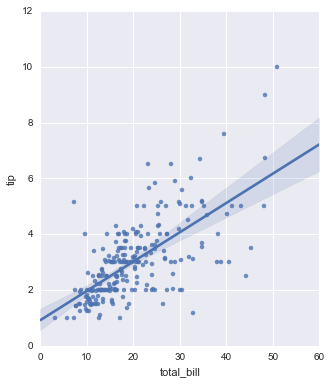
\includegraphics[width=0.55\linewidth]{images/regression_46_0}
	\end{figure}
\end{frame}
%===========================================================%
\begin{frame}[fragile]
	\frametitle{Seaborn Workshop}
	\large
	\begin{itemize}
		\item In contrast, the size and shape of the \texttt{lmplot()} figure is controlled through the \texttt{FacetGrid} interface using the size and aspect parameters, which apply to each facet in the plot, not to the overall figure itself:
	\end{itemize}
	
\end{frame}
%===========================================================%
\begin{frame}[fragile]
	\frametitle{Seaborn Workshop}
	\large
	\begin{verbatim}
	sns.lmplot(x="total_bill", y="tip", col="day", data=tips,
	col_wrap=2, size=3);
	\end{verbatim}
	
	\begin{figure}
		\centering
		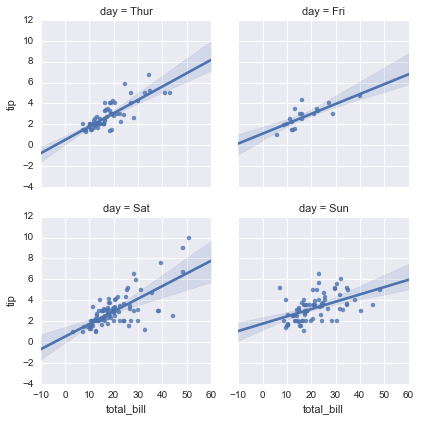
\includegraphics[width=0.55\linewidth]{images/regression_48_0}
	\end{figure}
\end{frame}
%===========================================================%
\begin{frame}[fragile]
	\frametitle{Seaborn Workshop}
	\large
	\begin{verbatim}
	sns.lmplot(x="total_bill", y="tip", col="day", data=tips,
	aspect=.5);
	\end{verbatim}
	
	\begin{figure}
		\centering
		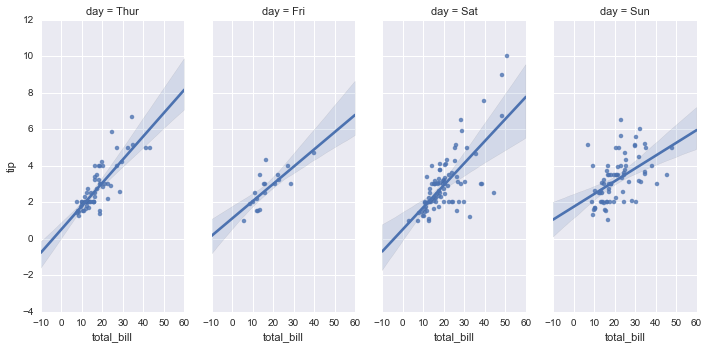
\includegraphics[width=0.7\linewidth]{images/regression_49_0}
	\end{figure}
	%============================================================%
\end{frame}
\section{Plotting a regression in other contexts}
%===========================================================%
\begin{frame}[fragile]
	\frametitle{Seaborn Workshop}
	\large
	\noindent \textbf{Plotting a regression in other contexts}
	\begin{itemize}
		\item A few other seaborn functions use \texttt{regplot()} in the context of a larger, more complex plot. 
		\item The first is the \texttt{jointplot()} function that we introduced in the distributions tutorial.
		\item In addition to the plot styles previously discussed, \texttt{jointplot()} can use \texttt{regplot()} to show the linear regression fit on the joint axes by passing \texttt{kind="reg"}:
	\end{itemize}
\end{frame}
%===========================================================%
\begin{frame}[fragile]
	\frametitle{Seaborn Workshop}
	\large
	
	\begin{verbatim}
	sns.jointplot(x="total_bill", y="tip", 
	data=tips, kind="reg");
	\end{verbatim}
	
	\begin{figure}
		\centering
		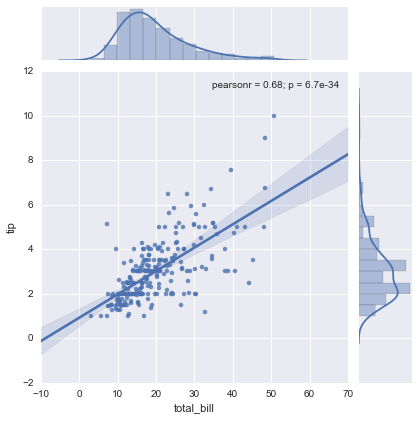
\includegraphics[width=0.60\linewidth]{images/regression_51_0}
	\end{figure}
\end{frame}
%===========================================================%
\begin{frame}[fragile]
	\frametitle{Seaborn Workshop}
	\large
	\begin{itemize}
		\item Using the \texttt{pairplot()} function with \texttt{kind="reg"} combines \texttt{regplot()} and \texttt{PairGrid} to show the linear relationship between variables in a dataset.
		\item Take care to note how this is different from \texttt{lmplot()}. 
		\item In the figure below, the two axes don’t show the same relationship conditioned on two levels of a third variable; rather, \item \texttt{PairGrid()} is used to show multiple relationships between different pairings of the variables in a dataset:
	\end{itemize}
	
\end{frame}
%===========================================================%
\begin{frame}[fragile]
	\large
	\begin{verbatim}
	sns.pairplot(tips, x_vars=["total_bill", "size"],  
	y_vars=["tip"], size=5, aspect=.8, kind="reg");
	\end{verbatim}
	\begin{figure}
		\centering
		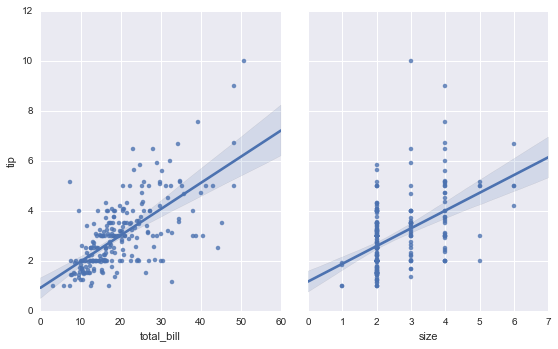
\includegraphics[width=0.8\linewidth]{images/regression_53_0}
	\end{figure}
	
\end{frame}
%===========================================================%
\begin{frame}[fragile]
	\frametitle{Seaborn Workshop}
	Like \texttt{lmplot()}, but unlike \texttt{jointplot()}, conditioning on an additional categorical variable is built into \texttt{pairplot()} using the hue parameter:
	
\end{frame}
%===========================================================%
\begin{frame}[fragile]
	\frametitle{Seaborn Workshop}
	\begin{verbatim}
	sns.pairplot(tips, x_vars=["total_bill", "size"], y_vars=["tip"],
	hue="smoker", size=5, aspect=.8, kind="reg");
	
	\end{verbatim}
	\begin{figure}
		\centering
		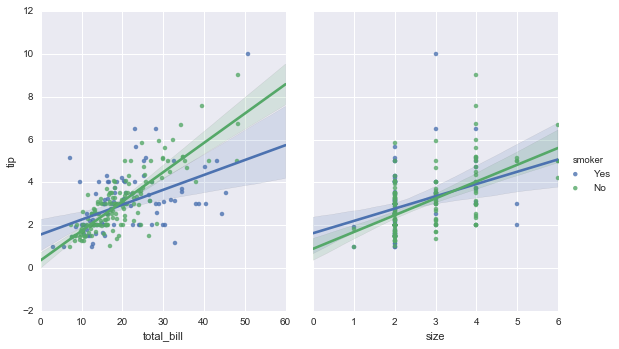
\includegraphics[width=0.8\linewidth]{images/regression_55_0}
	\end{figure}
\end{frame}
\end{document}